% \section{Моделирование токопереноса через ГС}
% \subsection{Алгоритм моделирования токопереноса через ГС}
% \begin{figure}[h]
%   \centering
%   \includegraphics[width=0.7\linewidth]{assets/AlgJ}
%   \caption{Блок схема алгорит моделирования токопереноса через ГС}
%   \label{img:AlgJ}
% \end{figure}

% \subsection{Результат моделирования}
% \begin{figure}[h]
%   \centering
%   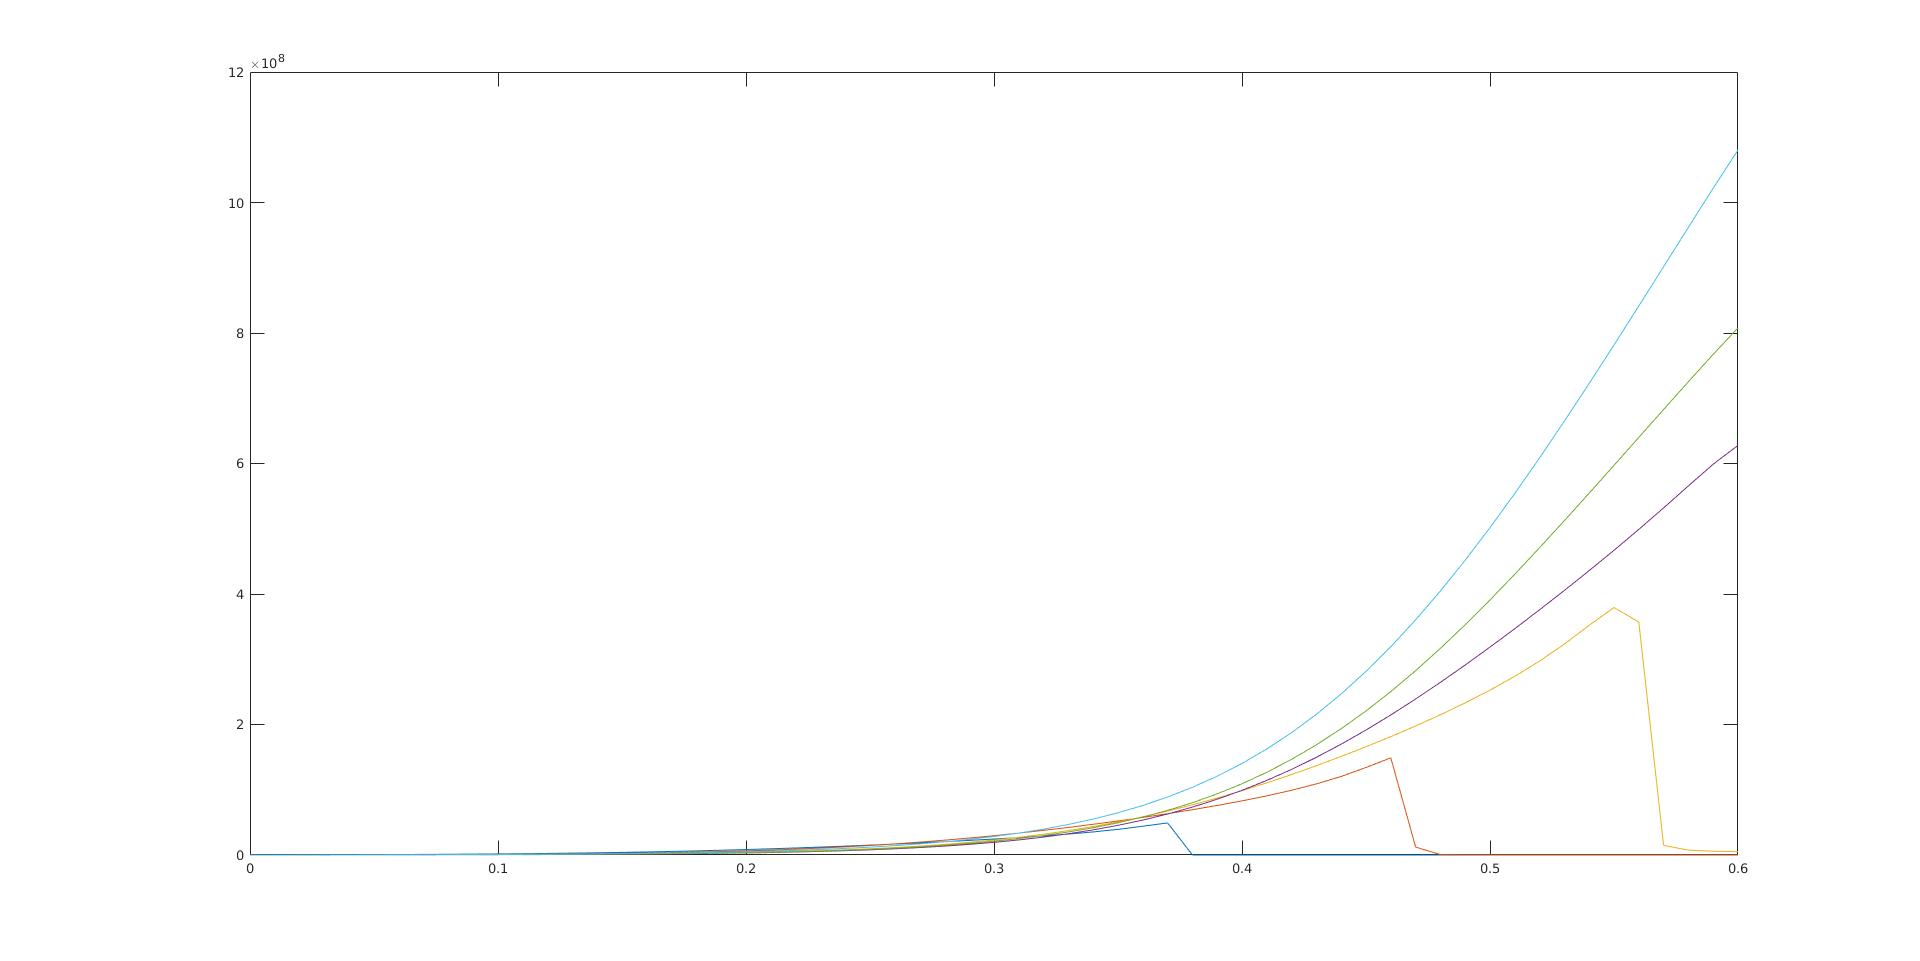
\includegraphics[width=1.1\linewidth]{assets/degrI25}
%   \caption{Результат моделирования токопереноса через гетероструктуру}
%   \label{img:degrI25}
% \end{figure}

\section{Моделирование диффузионного размытия $n^{+}\!-\!GaAs/i\!-\!GaAs/i\!-\!Al_{45}Ga_{55}As/ n^{+}\!-\!GaAs$}

\begin{figure}[h]
  \centering
  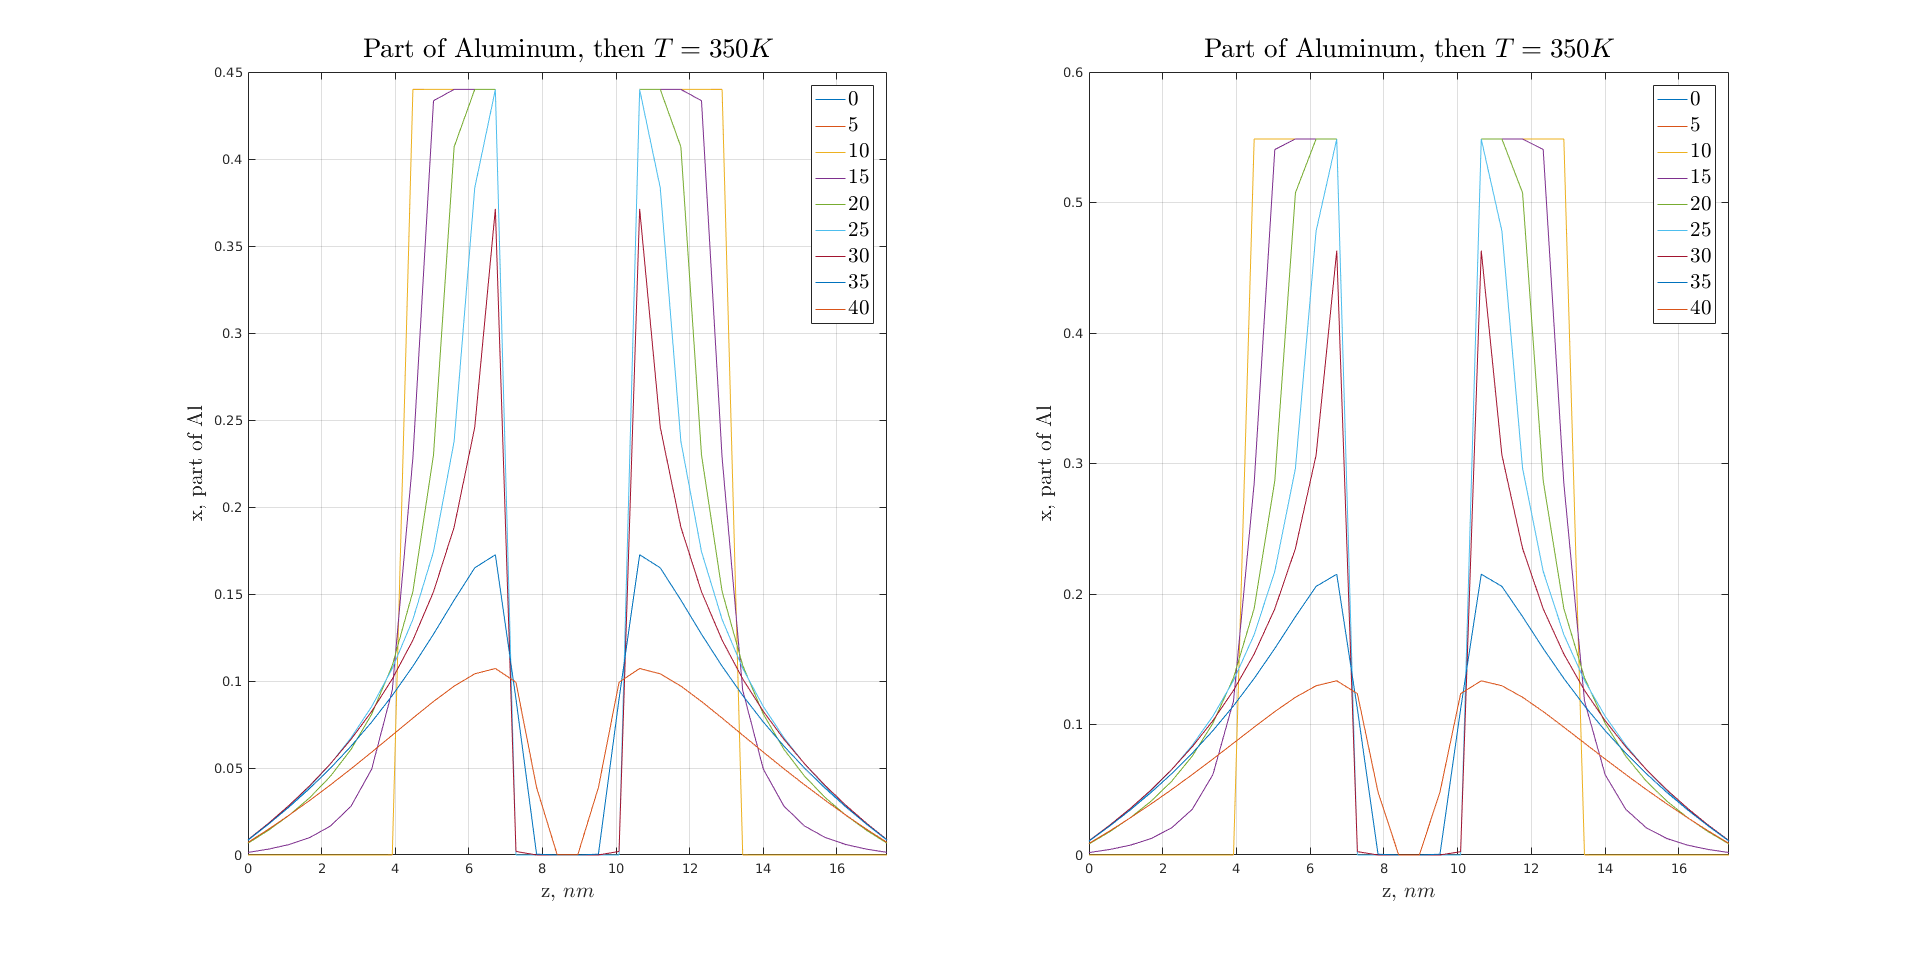
\includegraphics[width=0.9\linewidth]{DAlGaAs_Si}
  \caption{Диффузионное размытие}
\end{figure}

\begin{figure}[h]
  \centering
  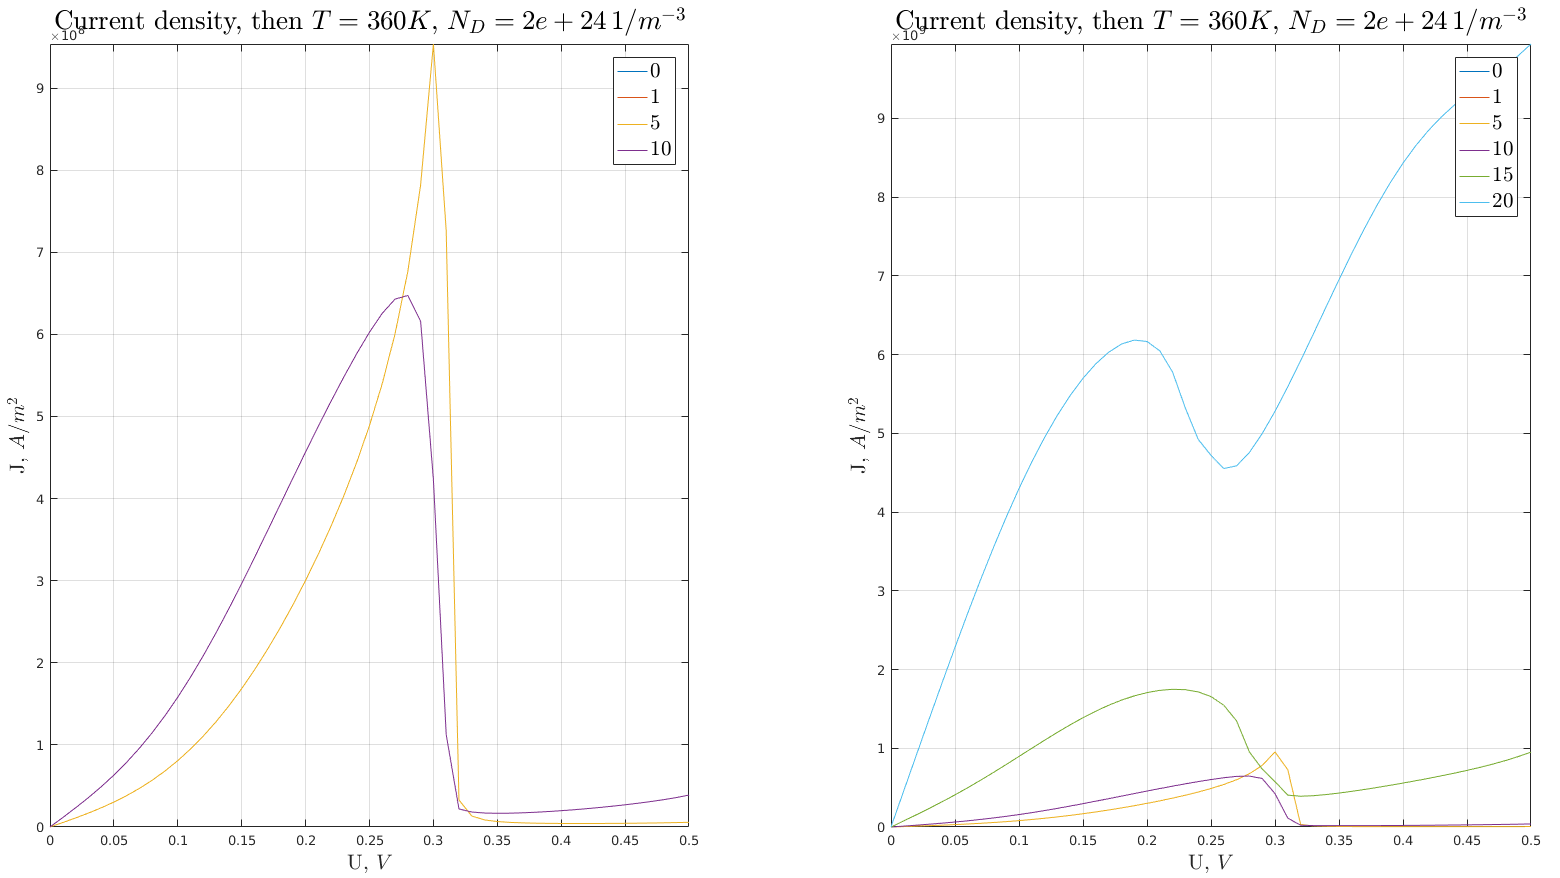
\includegraphics[width=0.9\linewidth]{JDAlGaAs_Si}
  \caption{Деградация ВАХ}
\end{figure}

\begin{figure}[h]
  \centering
  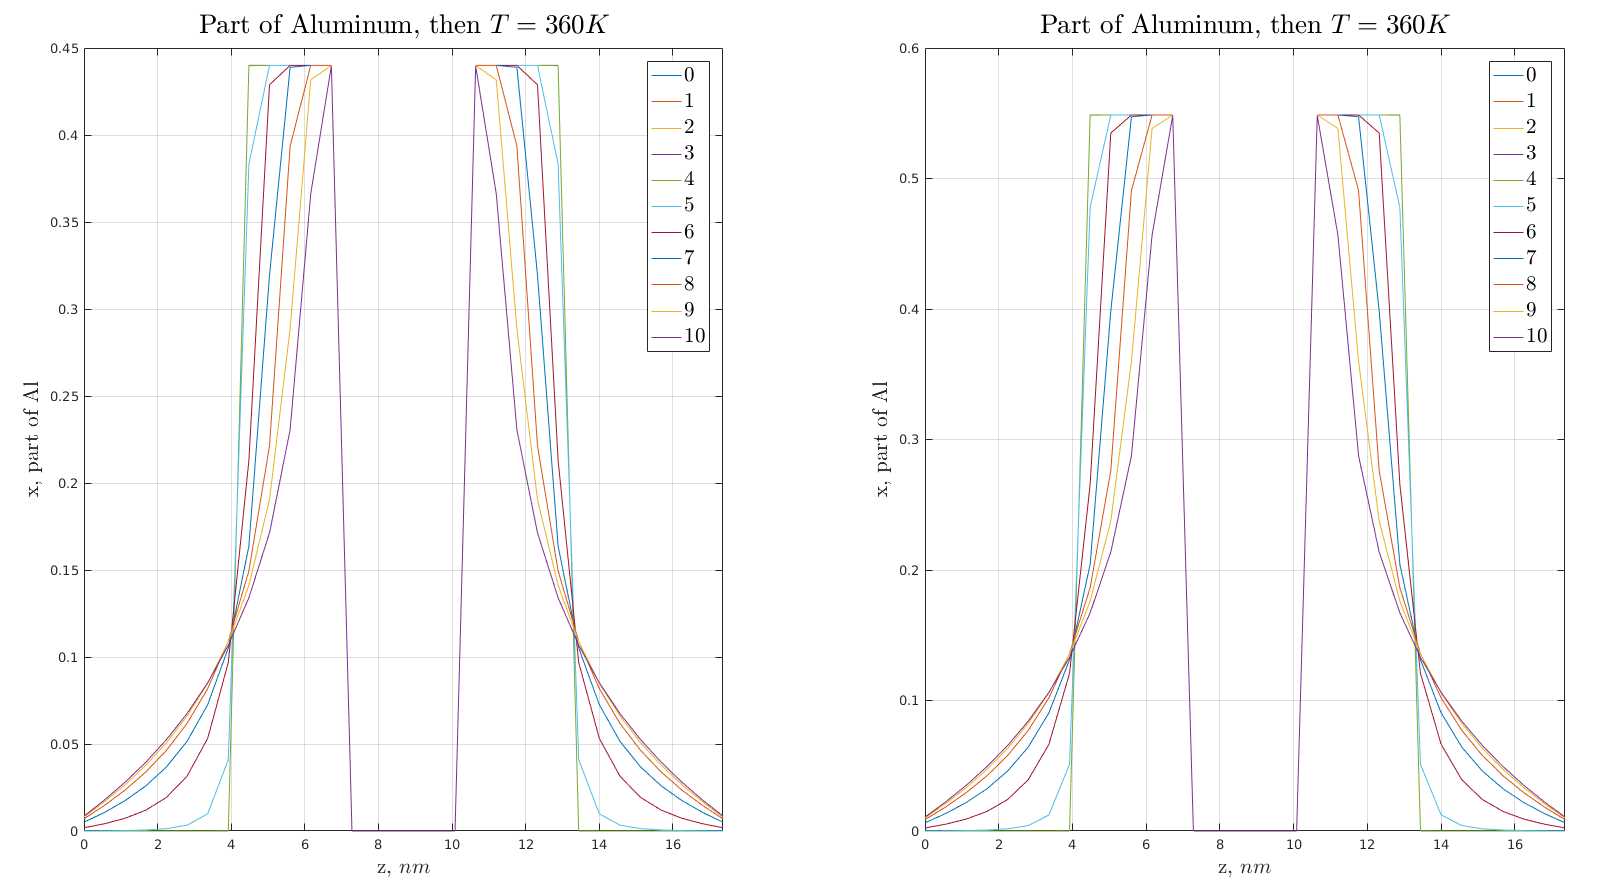
\includegraphics[width=\linewidth]{DAlGaAs_Si_360}
  \caption{Диффузионное размытие при повышении температуры}
\end{figure}

\begin{figure}[h]
  \centering
  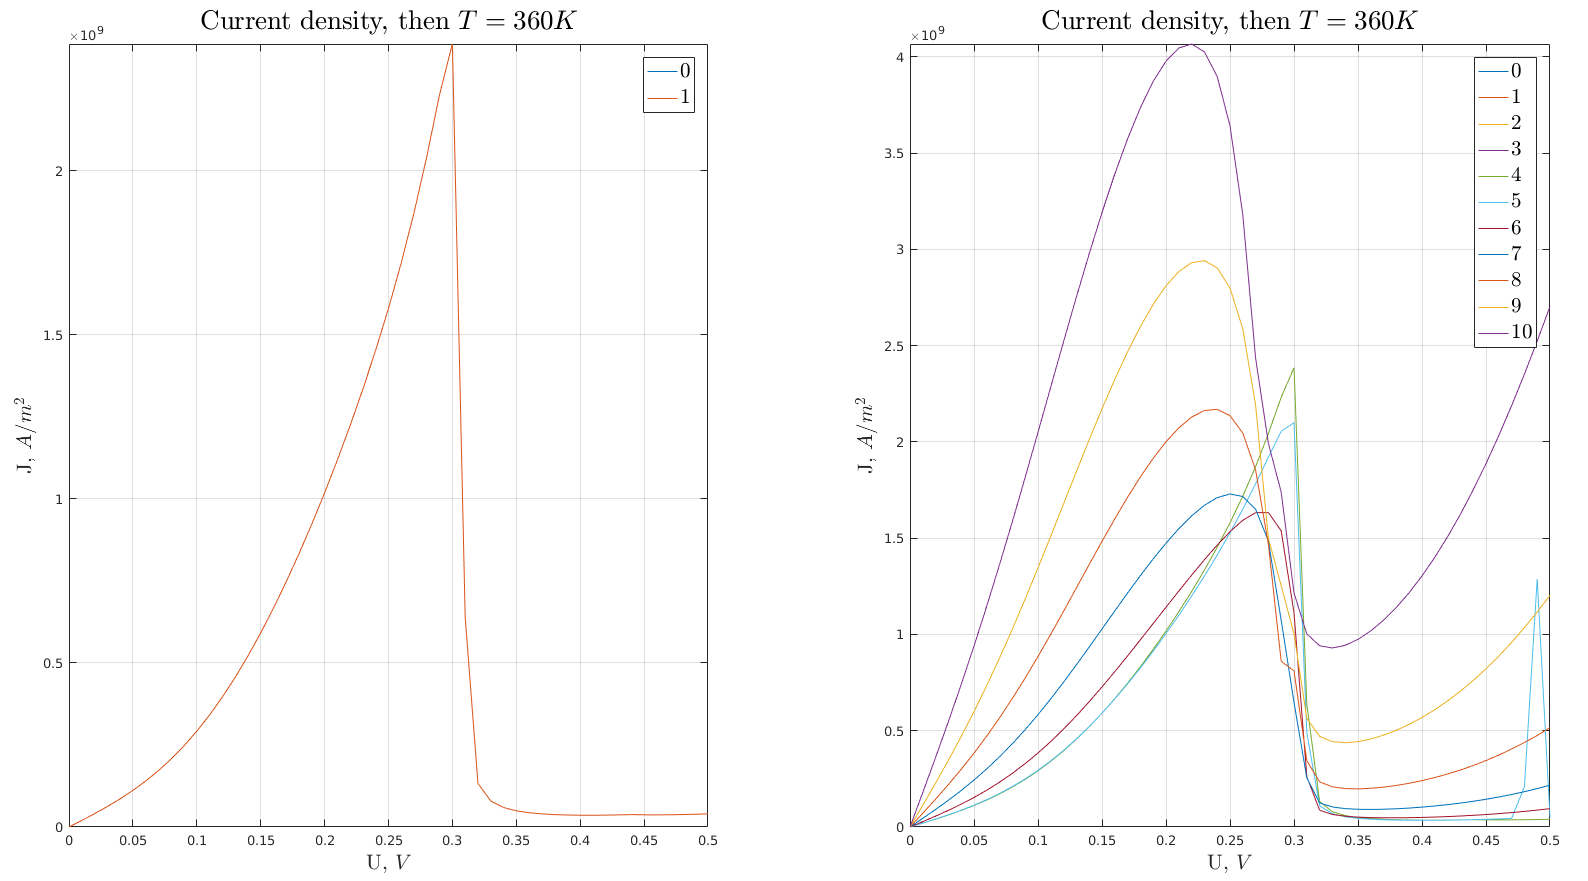
\includegraphics[width=\linewidth]{JDAlGaAs_Si_360}
  \caption{Деградация ВАХ при повышении температуры}
\end{figure}